\documentclass[../thesis]{subfiles}

\begin{document}
	\section{Further Optimizations}
	\label{sec:mic:further}

	The results obtained in the previous section prove that achieving higher efficiency with the coprocessor is not as trivial as porting the code for it. However, there are still unexplored paths, which will remain so in the context for this dissertation due to its natural time constraints. The most promising of these paths is the control of thread affinity in the \intel\xeonphi.

	One of the most problematic issues when using a \numa system lies in the fact that a process that starts in one processor may at some time be scheduled out and moved to another. The problem behind this lies in the memory hierarchy. When a process starts in a specific processor, it populates the cache and fills the memory directly linked to that processor with the data it requires. If moved to another processor, its data is no longer available in cache, which leads to a memory access, but the data it requires no longer lies in the closest memory. This also happens at the core level, with threads being scheduled to different cores inside the same processor, losing the advantage of locality in the core's private cache. For the specific case of \intel\mic devices, it is important for threads working with consecutive elements or in the same block to be in the same core for cache efficiency to be maximized.

	Although OpenMP (specification 3.1) does not include any way to control thread affinity, \intel's OpenMP library contains a mechanism for it through an environment variable (\texttt{KMP\_AFFINITY}) \cite{PRACE:MIC:BestPracticeGuide,CESGA:MIC:Evaluation}. \Cref{fig:kmp_affinity:balanced} shows the most promising affinity policy available in the coprocessor, where the threads are spread among the cores but grouped sequentially by ID when the number of demanded threads exceeds the number of cores. This policy is expected to achieve higher efficiency (due a better usage of the first levels of cache) with any granularity.

	\begin{figure}
		\begin{center}
			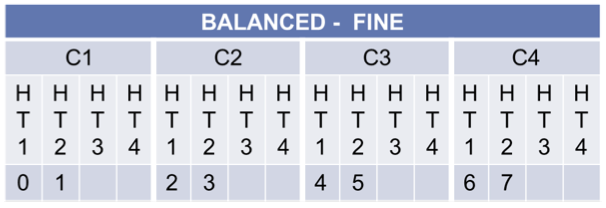
\includegraphics[width=0.7\textwidth]{assets/images/kmp_affinity_balanced.png}
		\end{center}
		\caption[Example of balanced thread affinity policy in (Intel OpenMP)]{Example of balanced thread affinity policy (Intel OpenMP) in a 4 core coprocessor for 8 threads with fine granularity}
		\label{fig:kmp_affinity:balanced}
	\end{figure}

	Despite this mechanism requiring minimal changes in the source code (or none at all), rerunning the performance tests at this point with the correct affinity setup would hamper the development of a \cuda implementation (described in the next chapter). Consequently, it is left for future work.

\end{document}
